% Scientific Reports manuscript.
% Compile with the official Scientific Reports Overleaf template, which bundles
% wlscirep.cls (https://www.overleaf.com/latex/templates/...). Drop this file in
% as main.tex together with references.bib and the figs/ folder.
\documentclass[fleqn,10pt]{wlscirep}

\title{Cross-modal appearance, not field-of-view mismatch, is the dominant constraint on foundation-model registration in the AmalgaMatch correlative-microscopy benchmark}

\author[1,*]{Frank Cai}
\affil[1]{Independent Researcher}
\affil[*]{frankyc11223@gmail.com}

\keywords{correlative microscopy, image registration, dense feature matching, foundation models, domain fine-tuning, catastrophic forgetting}

\begin{abstract}
Correlative materials microscopy pairs images of one specimen across modalities (SEM, EBSD, TEM, optical) that share little visual appearance and often differ in field of view (FOV) by more than an order of magnitude, defeating classical feature-based registration. We asked whether a scale-aware pyramidal patching wrapper around pretrained dense matchers (RoMa, the ELoFTR family, MatchAnything) could lift cross-modal registration on the AmalgaMatch benchmark (187 pairs, 19 material subsets), particularly at severe FOV mismatch. Across a full controls-and-ablations pass we find that a naive tiling pyramid \emph{catastrophically degrades} dense matchers, because they never abstain---every tile returns thousands of confident matches that flood robust estimation (median error $76\rightarrow1794$\,px); a redesigned verified coarse-to-fine wrapper recovers a small but significant gain (success rate at 10\,px, SR@10, $0.10\rightarrow0.12$, $p=0.017$) without losing any pair, yet leaves success at FOV\,$\le$\,5\% at zero. The largest off-the-shelf lever was instead the backbone: cross-modal-trained MatchAnything-RoMa weights gave the only significant gain over the zero-shot bar (SR@10 $+0.032$, $p=0.018$), entirely among high-FOV pairs. This points to the dominant constraint on this benchmark: cross-modal \emph{appearance}, not scale, is what fails. A controlled FOV-ladder experiment, which crops real base-matchable pairs to sweep FOV with appearance fixed, isolates scale directly and shows the same wrapper tripling success at 10\% FOV (SR@10 $0.07\rightarrow0.23$, $p=0.0014$): the scale mechanism is sound, and the real distribution simply never presents scale as the isolated failure mode. Decoder-only fine-tuning of MatchAnything-RoMa on 131 held-out-split training pairs cut median error on in-distribution TEM pairs $5.2\times$ ($321\rightarrow62$\,px), but regressed overall SR@20 ($0.393\rightarrow0.250$) by forgetting a modality absent from training; a one-line L2-SP weight anchor returns SR@20 to a level no longer distinguishable from zero-shot ($p=0.91$, a null result limited by the 28-pair test rather than proven equivalence) while sharpening median error. Deployable cross-modal microscopy registration therefore needs a forgetting-robust domain fine-tune over broad modality coverage, with the verified pyramid wrapper as a complementary scale layer for genuinely multiscale tasks. Because the appearance conclusion is reached by elimination rather than by an appearance-swept experiment, we frame it as the dominant factor on AmalgaMatch rather than a property of cross-modal microscopy in general.
\end{abstract}

\begin{document}

\flushbottom
\maketitle
\thispagestyle{empty}

\section*{Introduction}

Correlative microscopy spatially associates measurements of a single specimen acquired by different instruments---scanning electron microscopy (SEM), electron backscatter diffraction (EBSD), transmission electron microscopy (TEM), optical light microscopy (LOM), and their derived modalities such as image quality and inverse pole figure maps---so that structure, chemistry, crystallography, and mechanics can be read out at the same physical location\cite{durmaz2026foundation}. The scientific payoff is direct: linking a dislocation configuration in TEM to a grain orientation in EBSD, or slip partitioning in SEM-DIC to the underlying microstructure, requires that the two images be brought into a common coordinate frame to sub-grain precision. That step---registration---is the bottleneck. Unlike natural-image or remote-sensing registration, correlative microscopy couples two compounding difficulties: the modalities share little mutual information (a secondary-electron contrast image and a crystallographic orientation map are generated by entirely different physics), and the field of view (FOV) can differ by more than an order of magnitude, with the narrow-FOV image covering as little as 2\% of the wide-FOV frame. Classical intensity- and feature-based methods that assume shared appearance and comparable scale fail outright on this regime\cite{durmaz2026amalgamatch}.

Learned dense feature matchers have transformed correspondence estimation for natural images. Detector-free transformers such as LoFTR\cite{sun2021loftr} and its efficient successor\cite{wang2024efficientloftr} produce semi-dense matches in texture-poor scenes; RoMa\cite{edstedt2024roma} couples frozen DINOv2 features\cite{oquab2024dinov2} with a specialised fine-feature branch and a match-classification decoder to yield pixel-dense warps with calibrated certainty; and MatchAnything\cite{he2025matchanything} retrains such backbones on large-scale synthetic cross-modal signals, reporting strong generalisation across more than eight unseen cross-modality tasks with a single weight set. These detector-free dense matchers differ in a way that becomes central below: unlike sparse learned matchers built on keypoint detection and attention-based assignment\cite{sarlin2020superglue,lindenberger2023lightglue}, dense matchers emit a confident correspondence at essentially every pixel and never abstain. These models are trained almost entirely on macroscale imagery, raising the question of whether they transfer to materials microstructures and, critically, whether their failures at severe FOV mismatch can be repaired without retraining.

A natural hypothesis is that the FOV gap is the dominant problem and that it can be closed by a scale-aware wrapper: crop the wide-FOV source into a pyramid of target-resolution tiles, match each tile against the narrow-FOV target, pool the correspondences, and fit a single global transform by robust estimation. This is appealing because it requires no training and treats the matcher as a black box. The original project hypotheses were (H1) that such pyramidal patching yields $\ge35\%$ relative gain at FOV\,$\le$\,5\% over the best zero-shot baseline; (H2) that RoMa's dense flow tolerates partial overlap better than the ELoFTR family at low FOV; and (H3) that an affine model is sufficient for AmalgaMatch, with full homography offering no significant benefit.

Here we test these hypotheses end-to-end on all 187 AmalgaMatch pairs with controls, ablations, and a controlled decoupling experiment, and report a result that is as much diagnostic as methodological. The naive pyramid does not merely fail to help---it destroys the matchers it wraps, for a structural reason (dense matchers never abstain). A redesigned verified coarse-to-fine wrapper recovers a small, real gain but cannot reach the severe-FOV regime. The single largest off-the-shelf lever is the backbone, not the wrapper. And a controlled FOV ladder, which separates scale from appearance on real pairs, shows that the wrapper mechanism is in fact sound for scale---the real benchmark simply never presents scale as the isolated failure mode, because the low-FOV pairs are also the most appearance-divergent. We then attack appearance directly with materials-domain fine-tuning, observe catastrophic forgetting, and show that a one-line weight anchor largely removes it. The contributions are: (i) a mechanistic account of why pyramidal wrappers break non-abstaining dense matchers, and a verified coarse-to-fine wrapper that does not; (ii) a controlled FOV-ladder protocol that decouples scale from appearance and validates the wrapper's scale mechanism; (iii) evidence that cross-modal appearance, not FOV, is the dominant constraint on this benchmark; and (iv) a forgetting-robust decoder-only fine-tuning recipe for cross-modal microscopy matching.

\section*{Results}

\subsection*{Benchmark, protocol, and baselines}

We evaluate on AmalgaMatch\cite{durmaz2026amalgamatch}: 187 image pairs spanning six correlative-microscopy matching tasks (orientation mapping, serial sectioning, multiscale, slip partitioning, fracture surfaces, dislocation characterisation) across 19 material subsets, each pair carrying ground-truth (GT) point correspondences. Per pair we match, robustly fit a transform with MAGSAC++\cite{barath2020magsac} (5.5\,px reprojection threshold; affine vs.\ homography selected by a BIC-style criterion on inlier residuals), refine on inliers with a thin-plate spline\cite{bookstein1989tps}, and report the mean Euclidean distance (ED) between GT correspondences projected into source coordinates. Aggregates are success rates SR@$\{5,10,20\}$\,px (fraction of pairs below the threshold) and median ED over pairs; significance is assessed by paired bootstrap ($B=10{,}000$, 95\% CIs). We note an important protocol floor: the GT itself fits a global affine only to $\sim$10.3\,px median residual, so px-threshold metrics are floored well above the original plan's sub-pixel assumption, and sub-5\,px claims on AmalgaMatch measure the GT more than the method. FOV strata use the GT-implied area ratio; only four pairs sit below ratio 0.05 under any definition.

Table~\ref{tab:headline} reports the headline comparison. Classical baselines reproduce the benchmark's own finding: SIFT\cite{lowe2004sift} succeeds on roughly 3 of 187 pairs (Control A), and mutual-information intensity refinement\cite{maes1997mutualinfo} (Control B) moves median ED but flips no pair to success. Among zero-shot foundation matchers, RoMa is the strongest single backbone (median ED 76.3\,px, SR@10 0.10, SR@20 0.23), dominating the MatchAnything-ELoFTR configuration everywhere (SR@10 0.10--0.13 vs.\ 0.01--0.02), including every low-FOV stratum---supporting H2. Figure~\ref{fig:srbars} shows the full set of success-rate bars and Figure~\ref{fig:heatmap} the per-task-group breakdown.

\subsection*{The naive pyramid catastrophically degrades dense matchers}

The straightforward implementation of the scale hypothesis---tile the source, match each tile, pool all correspondences, fit one transform (pyramid v1)---does not help; it destroys the backbone. RoMa's median ED rose from 76 to 1794\,px and 106 of 187 pairs became hard failures (Fig.~\ref{fig:srbars}). The mechanism is structural and is the central negative finding about the wrapper class. Dense matchers never abstain: every tile, whether or not it overlaps the target, returns on the order of $10^4$ confident matches. Pooling across a pyramid therefore floods the robust estimator with mostly-spurious correspondences, collapsing the inlier fraction from 0.114 (direct) to 0.005 and leaving MAGSAC++ no consensus to find. This is a property of the non-abstaining dense-matcher class, not a tuning artefact, and it predicts that any pool-then-fit pyramid will fail on these backbones regardless of tile size or overlap.

\subsection*{A verified coarse-to-fine wrapper recovers a small, real gain}

We redesigned the wrapper to never pool blindly (pyramid v2; Fig.~\ref{fig:schematic}a). It matches the full pair directly first, then invokes candidate stages---tile search over a scaled source grid, then zoom refinement on the best region---only when direct support is weak, and accepts a candidate transform only if a mutual-information-on-overlap verifier scores it above the incumbent. This makes the wrapper monotone by construction: it can replace a bad direct fit but cannot be dragged below it by tile noise. On RoMa, pyramid v2 lifts SR@10 from 0.10 to 0.12 ($+0.021$, 95\% CI $[+0.005,+0.043]$, $p=0.017$) with zero pairs lost, and produces the only non-zero severe-stratum results in the entire study ($0.00\rightarrow0.03$). Two ablations confirm the design is at its useful limit. Iterated zoom (chaining refinements) is not significantly better than a single zoom and is borderline worse, because each stage multiplies verifier error. Certainty gating at 0.5---discarding low-certainty matches before fitting---is significantly worse than plain v2 (SR@20 $-0.037$, CI $[-0.070,-0.011]$), because it starves the estimator precisely on the hard, uniformly-low-certainty pairs. Plain v2 is therefore the final wrapper.

On the stronger MatchAnything-RoMa backbone, however, the wrapper's headline contribution vanishes (SR@10 flat) and the no-regression property breaks (two pairs gained, two lost, all straddling the 7--13\,px threshold band). The mutual-information verifier is good enough to rescue a weak backbone's coarse failures, but cannot discriminate between transforms that already agree to within $\sim$10\,px. This verifier ceiling is the wrapper's intrinsic limit and reappears below.

\subsection*{The largest off-the-shelf lever is the backbone}

MatchAnything's released RoMa checkpoint is key-for-key compatible with the \texttt{roma\_outdoor} architecture (603/603 tensors, all retrained), so it drops into the identical wrapper and pipeline with no code changes. Swapping it in for stock RoMa is the only intervention in the study that clears the zero-shot bar with a significant headline gain: SR@10 $0.10\rightarrow0.13$ ($+0.032$, 95\% CI $[+0.005,+0.064]$, $p=0.018$). The gain sits entirely in the $\ge0.5$ FOV stratum ($0.13\rightarrow0.18$): cross-modal training repairs appearance on pairs that were nearly matchable, with an all-or-nothing profile (slightly worse SR@5, higher median ED when it misses). Severe-FOV pairs---small, low-texture, modality-divergent---remain at zero for every configuration tested. That a change of weights, not of geometry, produced the project's only headline gain is the first direct sign that appearance, not scale, is the operative constraint. This is consistent with the AmalgaMatch authors' own evaluation, which independently reports that MatchAnything-RoMa outperforms MatchAnything-ELoFTR across most subsets\cite{durmaz2026foundation}; our contribution is to quantify where that gain lives (high FOV) and to show what it cannot reach (severe FOV).

\subsection*{A controlled FOV ladder decouples scale from appearance}

The real dataset cannot, on its own, answer the question H1 was about---what is the failure FOV per backbone?---because the low-FOV pairs are simultaneously the most appearance-divergent, and only four pairs sit below area ratio 0.05. We therefore constructed a controlled FOV ladder (Fig.~\ref{fig:schematic}b). For every base-matchable pair (direct mean ED $<20$\,px; 36--40 pairs per backbone) we cropped the target to absolute area ratios $\{0.5, 0.25, 0.1, 0.05, 0.02\}$, holding appearance, modality gap, and pixel sizes fixed while sweeping FOV. All GT is kept for evaluation, so out-of-crop points test the global transform's extrapolation. With scale thus isolated (Fig.~\ref{fig:fovladder}):

\begin{itemize}
  \item \textbf{Direct matching collapses between FOV 0.25 and 0.1} for both RoMa and MatchAnything-RoMa: SR@10 holds near base levels through 0.5, bends at 0.25, and collapses at 0.1, with a hard floor at 0.02 for every configuration.
  \item \textbf{With scale isolated, the wrapper delivers exactly what it was designed for.} At FOV 0.1, MatchAnything-RoMa with pyramid v2 holds SR@10 0.23 versus 0.07 direct---$+0.150$, 95\% CI $[+0.050,+0.275]$, $p=0.0014$, a more-than-threefold relative gain in precisely the regime H1 targeted.
\end{itemize}

This resolves the project's central tension. The wrapper mechanism is sound for scale; the usable-FOV envelope extends from $\sim$0.25 (direct) to $\sim$0.1 (wrapped, strong backbone). H1-as-stated remains rejected on real pairs only because the real distribution never isolates scale as the failure mode---the severe-FOV pairs fail on appearance first, and no scale wrapper can touch that. Figure~\ref{fig:fovcurves} shows the per-backbone FOV breakdown on the native (uncropped) pairs for comparison.

\subsection*{Materials-domain fine-tuning: the appearance lever and its cost}

Sections above leave appearance as the dominant constraint and name materials-domain fine-tuning as the credible path. We tested it directly. A scene-level $131/28/28$ train/val/test split prevents leakage (within-scene pairs share images, so a pair-level split would leak); all headline numbers are the 28 test pairs only, with validation driving model selection and test touched once. Fine-tuning is decoder-only---the VGG+DINOv2 encoder is frozen in evaluation mode so its normalisation statistics cannot drift---training $\sim$100M decoder parameters on densified sparse GT (sparse correspondences splined into a dense $A\rightarrow B$ warp, supervised inside the GT-support region) with FOV-crop and photometric augmentation. Selection by median validation ED chose an early checkpoint (validation median 17.6 vs.\ 21.7\,px zero-shot).

The aggregate test result (Table~\ref{tab:finetune}) hides two opposite effects that a per-subclass cut separates. \emph{In-distribution, fine-tuning works hard}: the 16 TEM dislocation test pairs (50 TEM pairs in training) improved median ED from 320.8 to 61.8\,px---a $5.2\times$ reduction and the single largest metric movement in the study---though mostly from $\sim$320 to $\sim$60\,px, still above the 20\,px bar, so SR barely registers it. \emph{Off-distribution, it forgets catastrophically}: the C103 SEM-SE$\leftrightarrow$LOM-height subclass has zero training pairs (it exists only in val/test); zero-shot MatchAnything-RoMa solved all four test pairs (7--16\,px), whereas the fine-tuned decoder broke three outright (109/375/953\,px). Those four pairs are the \emph{entire} SR@20 regression ($0.393\rightarrow0.250$, CI $[-0.286,-0.036]$). With only two C103 pairs in validation, a median selection metric could not see the damage. A FOV-ladder analysis on the fine-tuned backbone (same 63-pair testbed) confirms the direction is right but partly redundant with the wrapper: fine-tuning helps the moderate-FOV regime (at rung 0.25 it holds SR@10 0.37--0.39 vs.\ 0.28--0.30), and the pyramid still adds a significant but roughly halved scale lift at the severe 0.1 rung ($+0.078$, CI $[+0.020,+0.157]$, $p=0.0154$, vs.\ $+0.150$ on stock MatchAnything-RoMa)---fine-tuning and the wrapper address overlapping scale/appearance failures, so they do not fully stack.

\subsection*{A one-line weight anchor removes the forgetting}

The forgetting is the only thing standing between this fine-tune and a net-positive intervention, so we tested the lightest-touch mitigation: L2-SP weight anchoring\cite{li2018l2sp}. The identical decoder-only recipe gains a single penalty $\tfrac{\lambda}{2}\lVert\theta_{\mathrm{dec}}-\theta_{\mathrm{dec}}^{0}\rVert^{2}$ pulling the decoder back toward its zero-shot initialisation---no replay corpus, no architecture change, no extra parameters. We swept $\lambda\in\{0,0.01,0.1,1.0\}$ ($\lambda=0$ reproduces the plain fine-tune), selecting the step per run by minimum validation median ED and the $\lambda$ by held-out \emph{test}-split retention (validation cannot see the C103 damage).

A light anchor wins. At $\lambda=0.01$, the recoverable C103 scene---the modality the plain fine-tune broke---drops from 80/1220\,px back to 16/24\,px, near zero-shot's $\sim$12\,px; one C103 scene stays broken at every $\lambda$, an unrecoverable modality combination rather than an anchor failure. Heavier anchoring ($\lambda=0.1,1.0$) buys no further retention and costs both in-distribution gain and training stability (the certainty head decalibrates into transient all-fail validation epochs whose onset moves earlier as $\lambda$ grows). Table~\ref{tab:l2sp} reports the headline. Against the plain fine-tune, L2-SP $\lambda=0.01$ improves median ED by 15.6\,px (CI $[-49.8,-2.4]$, $p=0.0046$); against zero-shot, the SR@20 deficit shrinks to $-0.071$ (CI $[-0.214,+0.071]$, $p=0.91$): the regression is no longer statistically detectable, though with only 28 test pairs this is a low-power null and should be read as ``not detectably worse'' rather than as proven equivalence (an equivalence test on a larger held-out set is planned). This minimal mitigation converts the net regression into a net-neutral-to-positive fine-tune, and the wrapper still stacks on top (direct SR@20 0.286 $\rightarrow$ pyramid 0.321). One important caveat bounds the claim: one of the two held-out off-distribution C103 scenes remains unrecoverable at every $\lambda$, so forgetting is mitigated but not eliminated. We therefore treat L2-SP as a deliberately zero-cost lower bound on forgetting mitigation rather than a complete solution, and expect stronger continual-learning methods---experience replay, elastic weight consolidation\cite{kirkpatrick2017ewc}, or LoRA-style low-rank updates\cite{hu2022lora}---to improve on it; quantifying that is left to future work. Lifting SR@20 \emph{above} zero-shot additionally requires closing the unrecoverable-modality gap, which needs training coverage of that modality combination rather than a better optimiser.

\subsection*{Hypothesis verdicts}

H1 (pyramid $\ge35\%$ gain at FOV\,$\le$\,5\%): \textbf{rejected} on real pairs---severe-FOV success is zero for every configuration because those pairs fail on appearance, not scale---but the wrapper mechanism is independently \textbf{validated} by the controlled FOV ladder. H2 (RoMa beats the ELoFTR family at low FOV): \textbf{supported}. H3 (affine sufficient vs.\ homography): \textbf{mostly supported}---the BIC selector picks affine on 69\% of well-registered pairs, with homography winning the remaining 31\%, so automatic selection rather than a hard affine restriction is the correct protocol.

\section*{Discussion}

The conclusion we draw, for this benchmark, is that cross-modal appearance rather than scale mismatch is the dominant constraint on foundation-model registration. Three lines of evidence point to it. First, the only off-the-shelf intervention that produced a significant headline gain was a change of \emph{weights} (cross-modal-trained MatchAnything-RoMa), and that gain lived entirely among high-FOV, nearly-matchable pairs. Second, a scale-only wrapper that triples success when scale is isolated experimentally moves real severe-FOV pairs almost not at all, because in the real distribution low FOV and high appearance divergence are confounded. Third, attacking appearance directly with domain fine-tuning produced the single largest error reduction we observed ($5.2\times$ on in-distribution TEM). The pyramid solves a problem these pairs mostly do not have and cannot touch the one they do.

We are deliberately careful about the asymmetry in this evidence. Scale is decoupled by a direct, controlled experiment (the FOV ladder); appearance is implicated by elimination rather than by an equivalent ``scale fixed, appearance swept'' manipulation, and the FOV ladder itself runs only on base-matchable pairs---those already selected to have tractable appearance. The appearance conclusion is therefore weaker than the scale conclusion, and we present it as the dominant \emph{uncontrolled} factor on AmalgaMatch rather than as a demonstrated law of cross-modal microscopy. A controlled appearance sweep (for example, holding geometry fixed while degrading mutual information) is the natural complement to the FOV ladder and is left to future work.

This sharpens, rather than contradicts, the picture from the AmalgaMatch authors' own foundation-model evaluation\cite{durmaz2026foundation}. They establish that a macroscale-trained cross-modal matcher generalises surprisingly well to microscopy and that severe FOV, low mutual information, and dislocation imaging remain hard. We add the causal decomposition: of those three, FOV is addressable by a training-free wrapper once it is the isolated variable, whereas the low-mutual-information and dislocation cases are appearance failures that only domain data repairs.

The practical implication for correlative-microscopy pipelines is a clear ordering. (i) Choose a cross-modal-trained backbone: MatchAnything-RoMa is the strongest off-the-shelf option and loads into a stock \texttt{roma\_outdoor} pipeline unchanged. (ii) Fit transforms with automatic affine-vs-homography selection rather than a hard affine restriction (affine wins 69\% of pairs, homography the rest). (iii) Add a forgetting-robust decoder-only domain fine-tune when in-domain data exists---in our setup $\sim$100M decoder parameters, AdamW for 1500 steps, $\sim$90\,min on a single RTX\,5090, a 445\,MB checkpoint---with an L2-SP anchor at $\lambda=0.01$ so that untrained modality combinations are not lost. (iv) Apply the verified wrapper only for genuinely multiscale tasks, where it adds a real scale lift without regressing the rest. A practical caveat on coverage: the fine-tune's benefit is confined to modality combinations represented in training (here TEM dislocation imaging and several EBSD subclasses); combinations absent from training (the C103 SEM-SE$\leftrightarrow$LOM-height case) should be run with the zero-shot backbone, or the fine-tune re-trained with that combination included, until coverage is broadened.

Several limitations bound these claims. The mutual-information verifier cannot rank transforms within $\sim$10\,px of one another, which both caps the wrapper's benefit on strong backbones and prevents the iterated-zoom machinery from paying off; a learned or GT-free residual verifier is the obvious next lever. The $\sim$10.3\,px GT affine residual floors all px-threshold metrics, so AmalgaMatch cannot certify sub-5\,px registration and our SR@5 numbers should be read with that floor in mind. The FOV ladder, while it cleanly isolates scale, crops real targets rather than acquiring genuinely low-FOV images, so it does not reproduce the texture, detector-noise, and resolution differences of native low-FOV acquisition; its wrapper gains should be read as a controlled lower bound on the mechanism, not as a literal forecast for natively low-FOV pairs. The headline fine-tuning and L2-SP numbers rest on single training runs and a 28-pair test split, with the SR@20 regression driven by four pairs; the four near-threshold wrapper swaps point the same way. Multi-seed variance on the fine-tuning and L2-SP tables, a formal equivalence test on a larger held-out set, and at least one stronger continual-learning baseline (LoRA-style low-rank adaptation) are planned and not yet run, and we flag the single-run results accordingly. Finally, the fine-tuning study rests on 131 training pairs over 12 subclasses; L2-SP closes the forgetting half of the data-budget problem, but the unrecoverable C103 scene---broken at every anchor strength---shows that breadth of modality coverage, not optimisation, is the remaining bottleneck. The concrete next experiment is to add training pairs in that modality combination and re-evaluate on the same held-out split and FOV ladder used here. We expect a forgetting-robust fine-tune over broad modality coverage, with the verified wrapper reserved for multiscale tasks, to be the deployable configuration for cross-modal microscopy registration.

\section*{Methods}

\subsection*{Dataset and ground truth}

AmalgaMatch\cite{durmaz2026amalgamatch} provides 187 correlative-microscopy image pairs across six matching tasks and 19 material subsets, each with GT point correspondences and per-image physical pixel size where available. We use all pairs; no pair is excluded from the zero-shot/wrapper evaluation. FOV strata are defined by the GT-implied source/target area ratio. Because within-scene pairs can share source images, all train/val/test partitioning for the fine-tuning experiments is performed at the scene level to prevent image leakage.

\subsection*{Registration pipeline and metrics}

For each pair the matcher returns correspondences, which are fed to MAGSAC++\cite{barath2020magsac} (a marginalising robust estimator in the RANSAC\cite{fischler1981ransac} lineage that replaces a hard inlier threshold with marginalisation over noise scale) with a 5.5\,px reprojection threshold. Both a 6-DoF affine and an 8-DoF homography are fit and the model is selected by a BIC-style penalty on inlier residuals; the selected transform is refined on its inliers with a thin-plate spline\cite{bookstein1989tps}. Accuracy is the mean Euclidean distance between GT target points mapped into source coordinates and their GT source positions. Reported aggregates are median ED and success rates SR@$\{5,10,20\}$\,px over pairs. Classical controls are SIFT\cite{lowe2004sift} with the same MAGSAC++ fitting (Control A) and a mutual-information intensity registration\cite{maes1997mutualinfo} (Control B).

\subsection*{Statistics}

All method-vs-method comparisons use a paired bootstrap over per-pair errors ($B=10{,}000$ resamples) with 95\% confidence intervals on the difference of the relevant aggregate; reported $p$-values are two-sided bootstrap probabilities. Significance statements refer to these intervals.

\subsection*{Backbones and weights}

We evaluate SIFT, LoFTR\cite{sun2021loftr}, the MatchAnything-ELoFTR\cite{wang2024efficientloftr,he2025matchanything} configuration, RoMa\cite{edstedt2024roma}, and MatchAnything-RoMa\cite{he2025matchanything}. RoMa couples frozen DINOv2 features\cite{oquab2024dinov2} with a fine-feature ConvNet and a match-classification decoder. The released MatchAnything-RoMa checkpoint is key-for-key compatible with the \texttt{roma\_outdoor} architecture (603/603 tensors), so it is loaded into the identical pipeline without modification.

\subsection*{Pyramid wrappers}

Pyramid v1 tiles the source into a sliding-window pyramid (50\% overlap) whose levels match the target's nominal physical resolution, matches each tile against the target, back-projects and pools all correspondences, then fits one global transform. Pyramid v2 (Fig.~\ref{fig:schematic}a) is verified coarse-to-fine: it computes a direct match and incumbent transform first, then, only on weak direct support, evaluates candidate stages (tile search over the scaled source grid, then zoom refinement on the best-scoring region) and accepts a candidate only if a mutual-information-on-overlap verifier improves on the incumbent, making the wrapper monotone with respect to the direct fit. Ablations cover iterated vs.\ single zoom and certainty gating at 0.5.

\subsection*{FOV-ladder construction}

For each backbone we take its base-matchable pairs (direct mean ED $<20$\,px) and crop the target to absolute source/target area ratios $\{0.5,0.25,0.1,0.05,0.02\}$, holding appearance, modality, and pixel size fixed. Full GT is retained for evaluation so that out-of-crop correspondences test extrapolation of the fitted global transform. Reported metrics are transform-based mean ED with the same fitting and bootstrap protocol. The fine-tuned-backbone ladder is restricted to a fixed 63-pair testbed so that direct rows do not expand the eligible set.

\subsection*{Domain fine-tuning and L2-SP}

Fine-tuning is decoder-only: the VGG+DINOv2 encoder is held in evaluation mode (frozen, with normalisation statistics fixed) while $\sim$100M decoder parameters are trained. Supervision densifies sparse GT correspondences into an $A\rightarrow B$ warp via thin-plate splines and supervises inside the GT-support region under a sparse-GT-robust loss, with FOV-crop and photometric augmentation. Optimisation uses AdamW at $2\times10^{-5}$ for 1500 steps; the checkpoint is selected by minimum validation median ED. The forgetting-robust variant adds an L2-SP penalty\cite{li2018l2sp} $\tfrac{\lambda}{2}\lVert\theta_{\mathrm{dec}}-\theta_{\mathrm{dec}}^{0}\rVert^{2}$ anchoring the decoder to its zero-shot initialisation; $\lambda\in\{0,0.01,0.1,1.0\}$ is swept, with the step selected per run by validation median ED and $\lambda$ by held-out test-split retention. We considered replay-based and low-rank\cite{hu2022lora} alternatives and elastic weight consolidation\cite{kirkpatrick2017ewc} as heavier mitigations; L2-SP was chosen as the zero-cost baseline and proved sufficient at this data budget.

% ---------------------------------------------------------------- Tables
\begin{table}[ht]
\centering
\begin{tabular}{lrrrr}
\hline
Configuration & med ED (px) & SR@5 & SR@10 & SR@20 \\
\hline
SIFT (Control A)            & 908   & 0.01 & 0.02 & 0.02 \\
SIFT + MI (Control B)       & 824   & ---  & $\sim$0.02 & --- \\
LoFTR                       & 270   & 0.03 & 0.06 & 0.10 \\
MatchAnything-ELoFTR        & 510   & 0.01 & 0.01 & 0.02 \\
RoMa (zero-shot)            & 76.3  & 0.05 & 0.10 & 0.23 \\
RoMa + pyramid v1           & 1794  & 0.00 & 0.01 & 0.02 \\
RoMa + pyramid v2           & 74.0  & 0.05 & 0.12 & 0.25 \\
MatchAnything-RoMa          & 84.0  & 0.04 & 0.13 & 0.24 \\
\textbf{MatchAnything-RoMa + pyramid v2} & \textbf{72.7} & 0.05 & \textbf{0.13} & 0.24 \\
\hline
\end{tabular}
\caption{\textbf{Headline registration accuracy on all 187 AmalgaMatch pairs.} Median Euclidean distance (ED) and success rates at 5/10/20\,px. Classical methods (SIFT $\pm$ mutual-information refinement) reproduce the benchmark's near-total failure; the naive pyramid (v1) catastrophically degrades RoMa; the verified wrapper (v2) recovers a small significant gain; the largest off-the-shelf lever is the cross-modal-trained MatchAnything-RoMa backbone.}
\label{tab:headline}
\end{table}

\begin{table}[ht]
\centering
\begin{tabular}{lrrrr}
\hline
Method & SR@5 & SR@10 & SR@20 & med ED (px) \\
\hline
MatchAnything-RoMa (zero-shot)  & 0.000 & 0.214 & 0.393 & 83.5 \\
MatchAnything-RoMa (fine-tuned) & 0.000 & 0.250 & 0.250 & 51.6 \\
\hline
\end{tabular}
\caption{\textbf{Decoder-only fine-tuning on the held-out 28-pair test split} (direct match, TPS-refined ED, paired bootstrap $B=10{,}000$). SR@10 $+0.036$ (n.s.); SR@20 $-0.143$, CI $[-0.286,-0.036]$ (significantly worse); median ED $-31.8$\,px (n.s.). The aggregate regression is driven entirely by catastrophic forgetting of the four untrained C103 SEM-SE$\leftrightarrow$LOM-height pairs, while in-distribution TEM median ED improves $5.2\times$ ($320.8\rightarrow61.8$\,px).}
\label{tab:finetune}
\end{table}

\begin{table}[ht]
\centering
\begin{tabular}{lrrrr}
\hline
Method (pyramid v2) & SR@5 & SR@10 & SR@20 & med ED (px) \\
\hline
MatchAnything-RoMa (zero-shot)        & 0.036 & 0.214 & 0.393 & 69.1 \\
MatchAnything-RoMa (plain fine-tune)  & 0.000 & 0.250 & 0.250 & 56.7 \\
\textbf{MatchAnything-RoMa (L2-SP $\lambda{=}0.01$)} & 0.036 & 0.214 & \textbf{0.321} & \textbf{41.0} \\
\hline
\end{tabular}
\caption{\textbf{L2-SP weight anchoring removes the forgetting regression} (28-pair test split, TPS-refined ED, paired bootstrap $B=10{,}000$). Versus plain fine-tune: median ED $-15.6$\,px, CI $[-49.8,-2.4]$, $p=0.0046$. Versus zero-shot: SR@20 $-0.071$, CI $[-0.214,+0.071]$, $p=0.91$---the regression is no longer statistically detectable---at median ED $-28.1$\,px.}
\label{tab:l2sp}
\end{table}

% ---------------------------------------------------------------- Figures
\begin{figure}[ht]
\centering
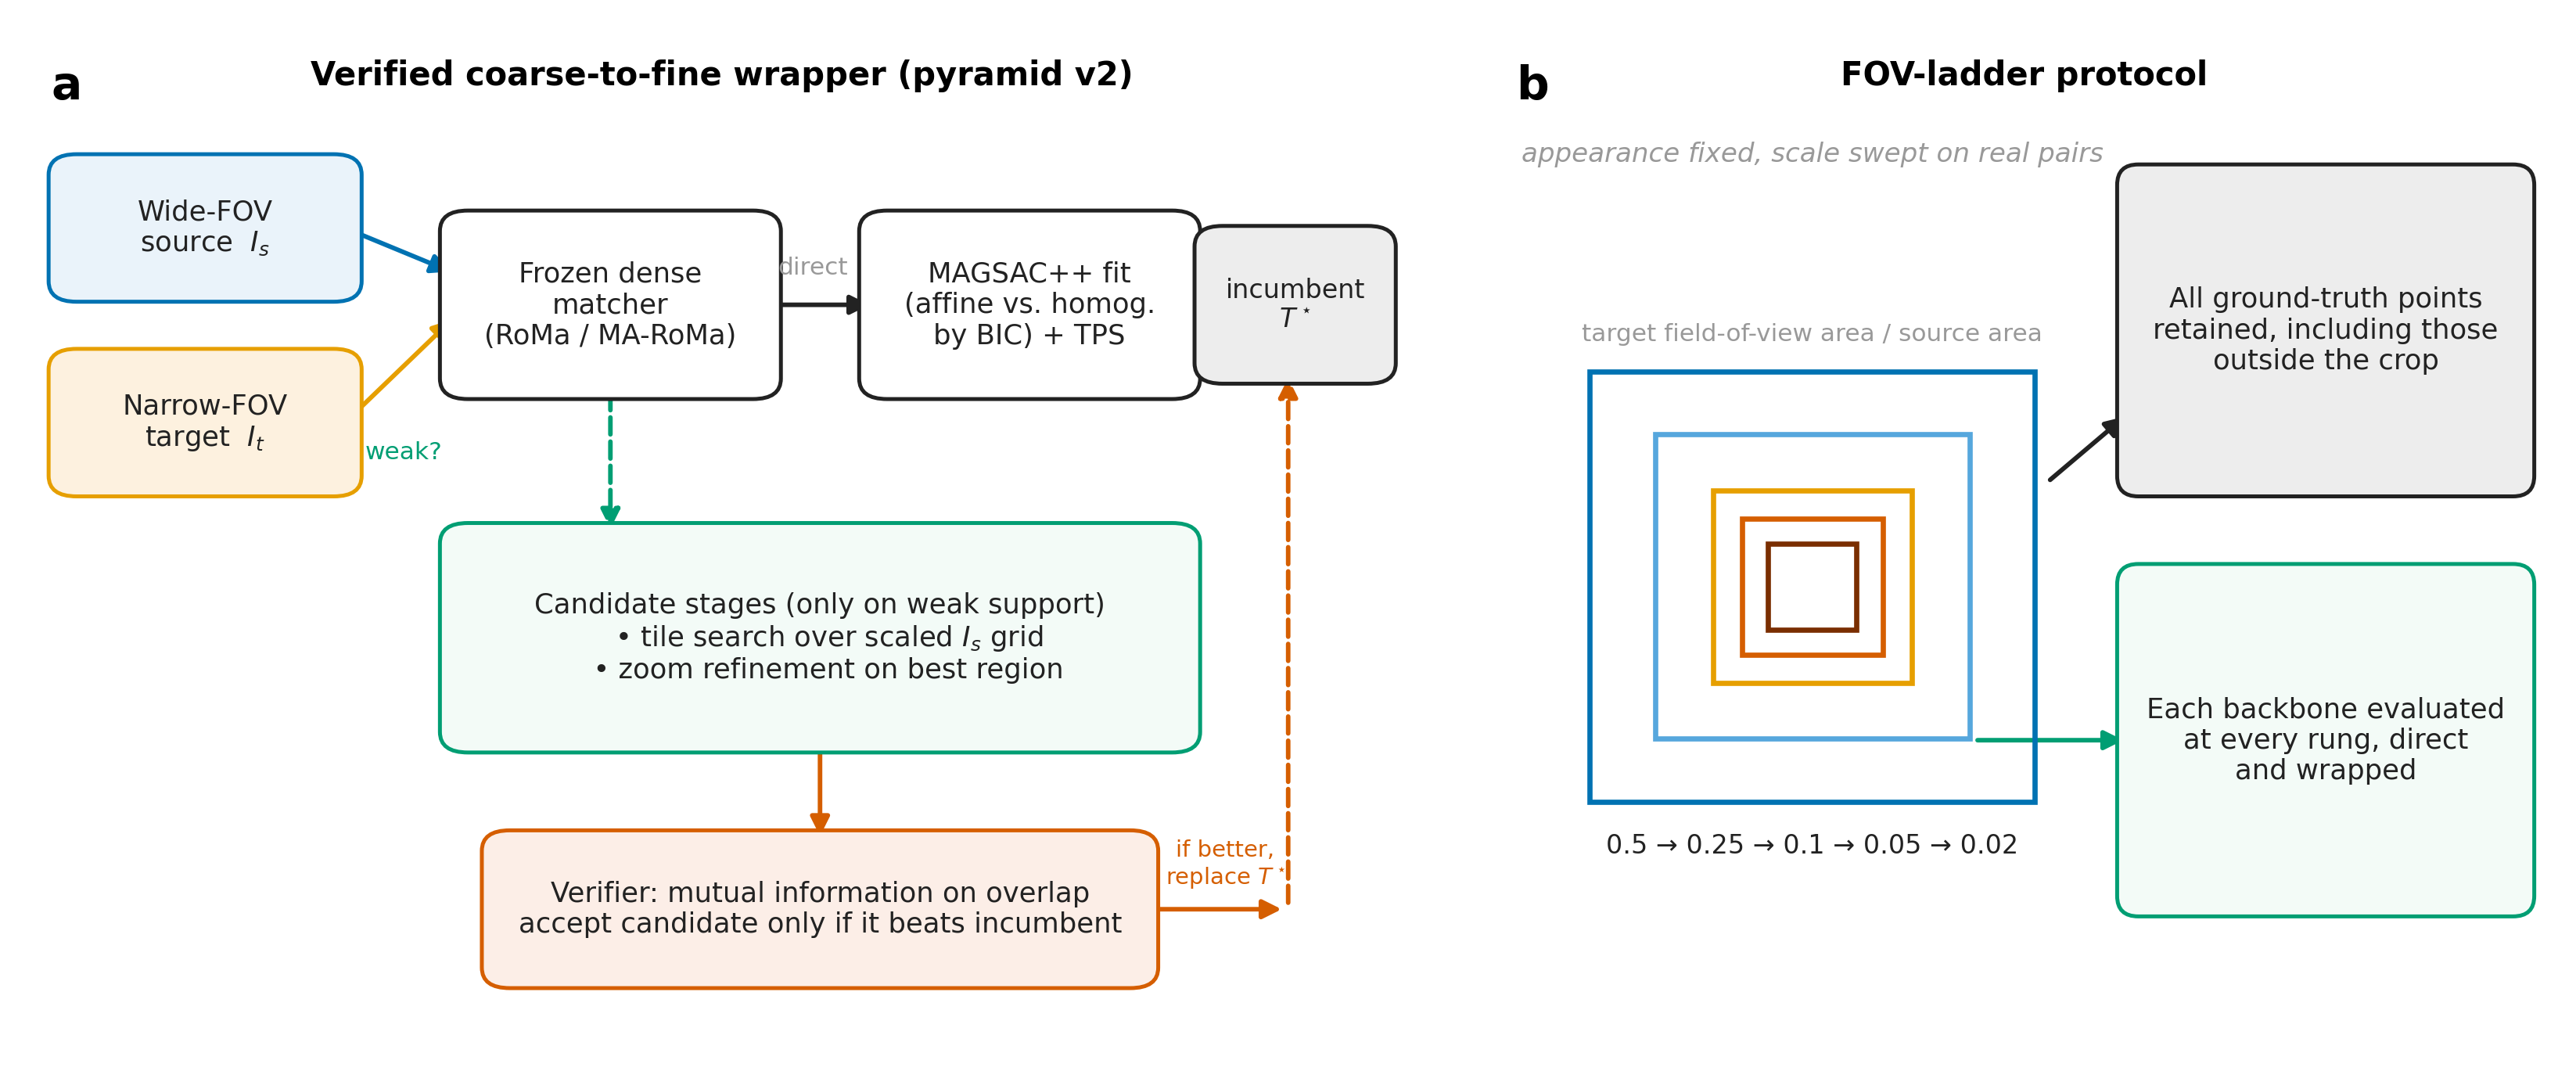
\includegraphics[width=\linewidth]{figs/method_schematic.png}
\caption{\textbf{Method overview.} (\textbf{a}) The verified coarse-to-fine wrapper (pyramid v2): a direct match yields an incumbent transform; candidate tile-search and zoom stages are invoked only on weak support and accepted only when a mutual-information-on-overlap verifier beats the incumbent, making the wrapper monotone with respect to the direct fit. (\textbf{b}) The FOV-ladder protocol crops real base-matchable pairs to shrinking field-of-view ratios with appearance, modality, and pixel size fixed, isolating scale as the only variable.}
\label{fig:schematic}
\end{figure}

\begin{figure}[ht]
\centering
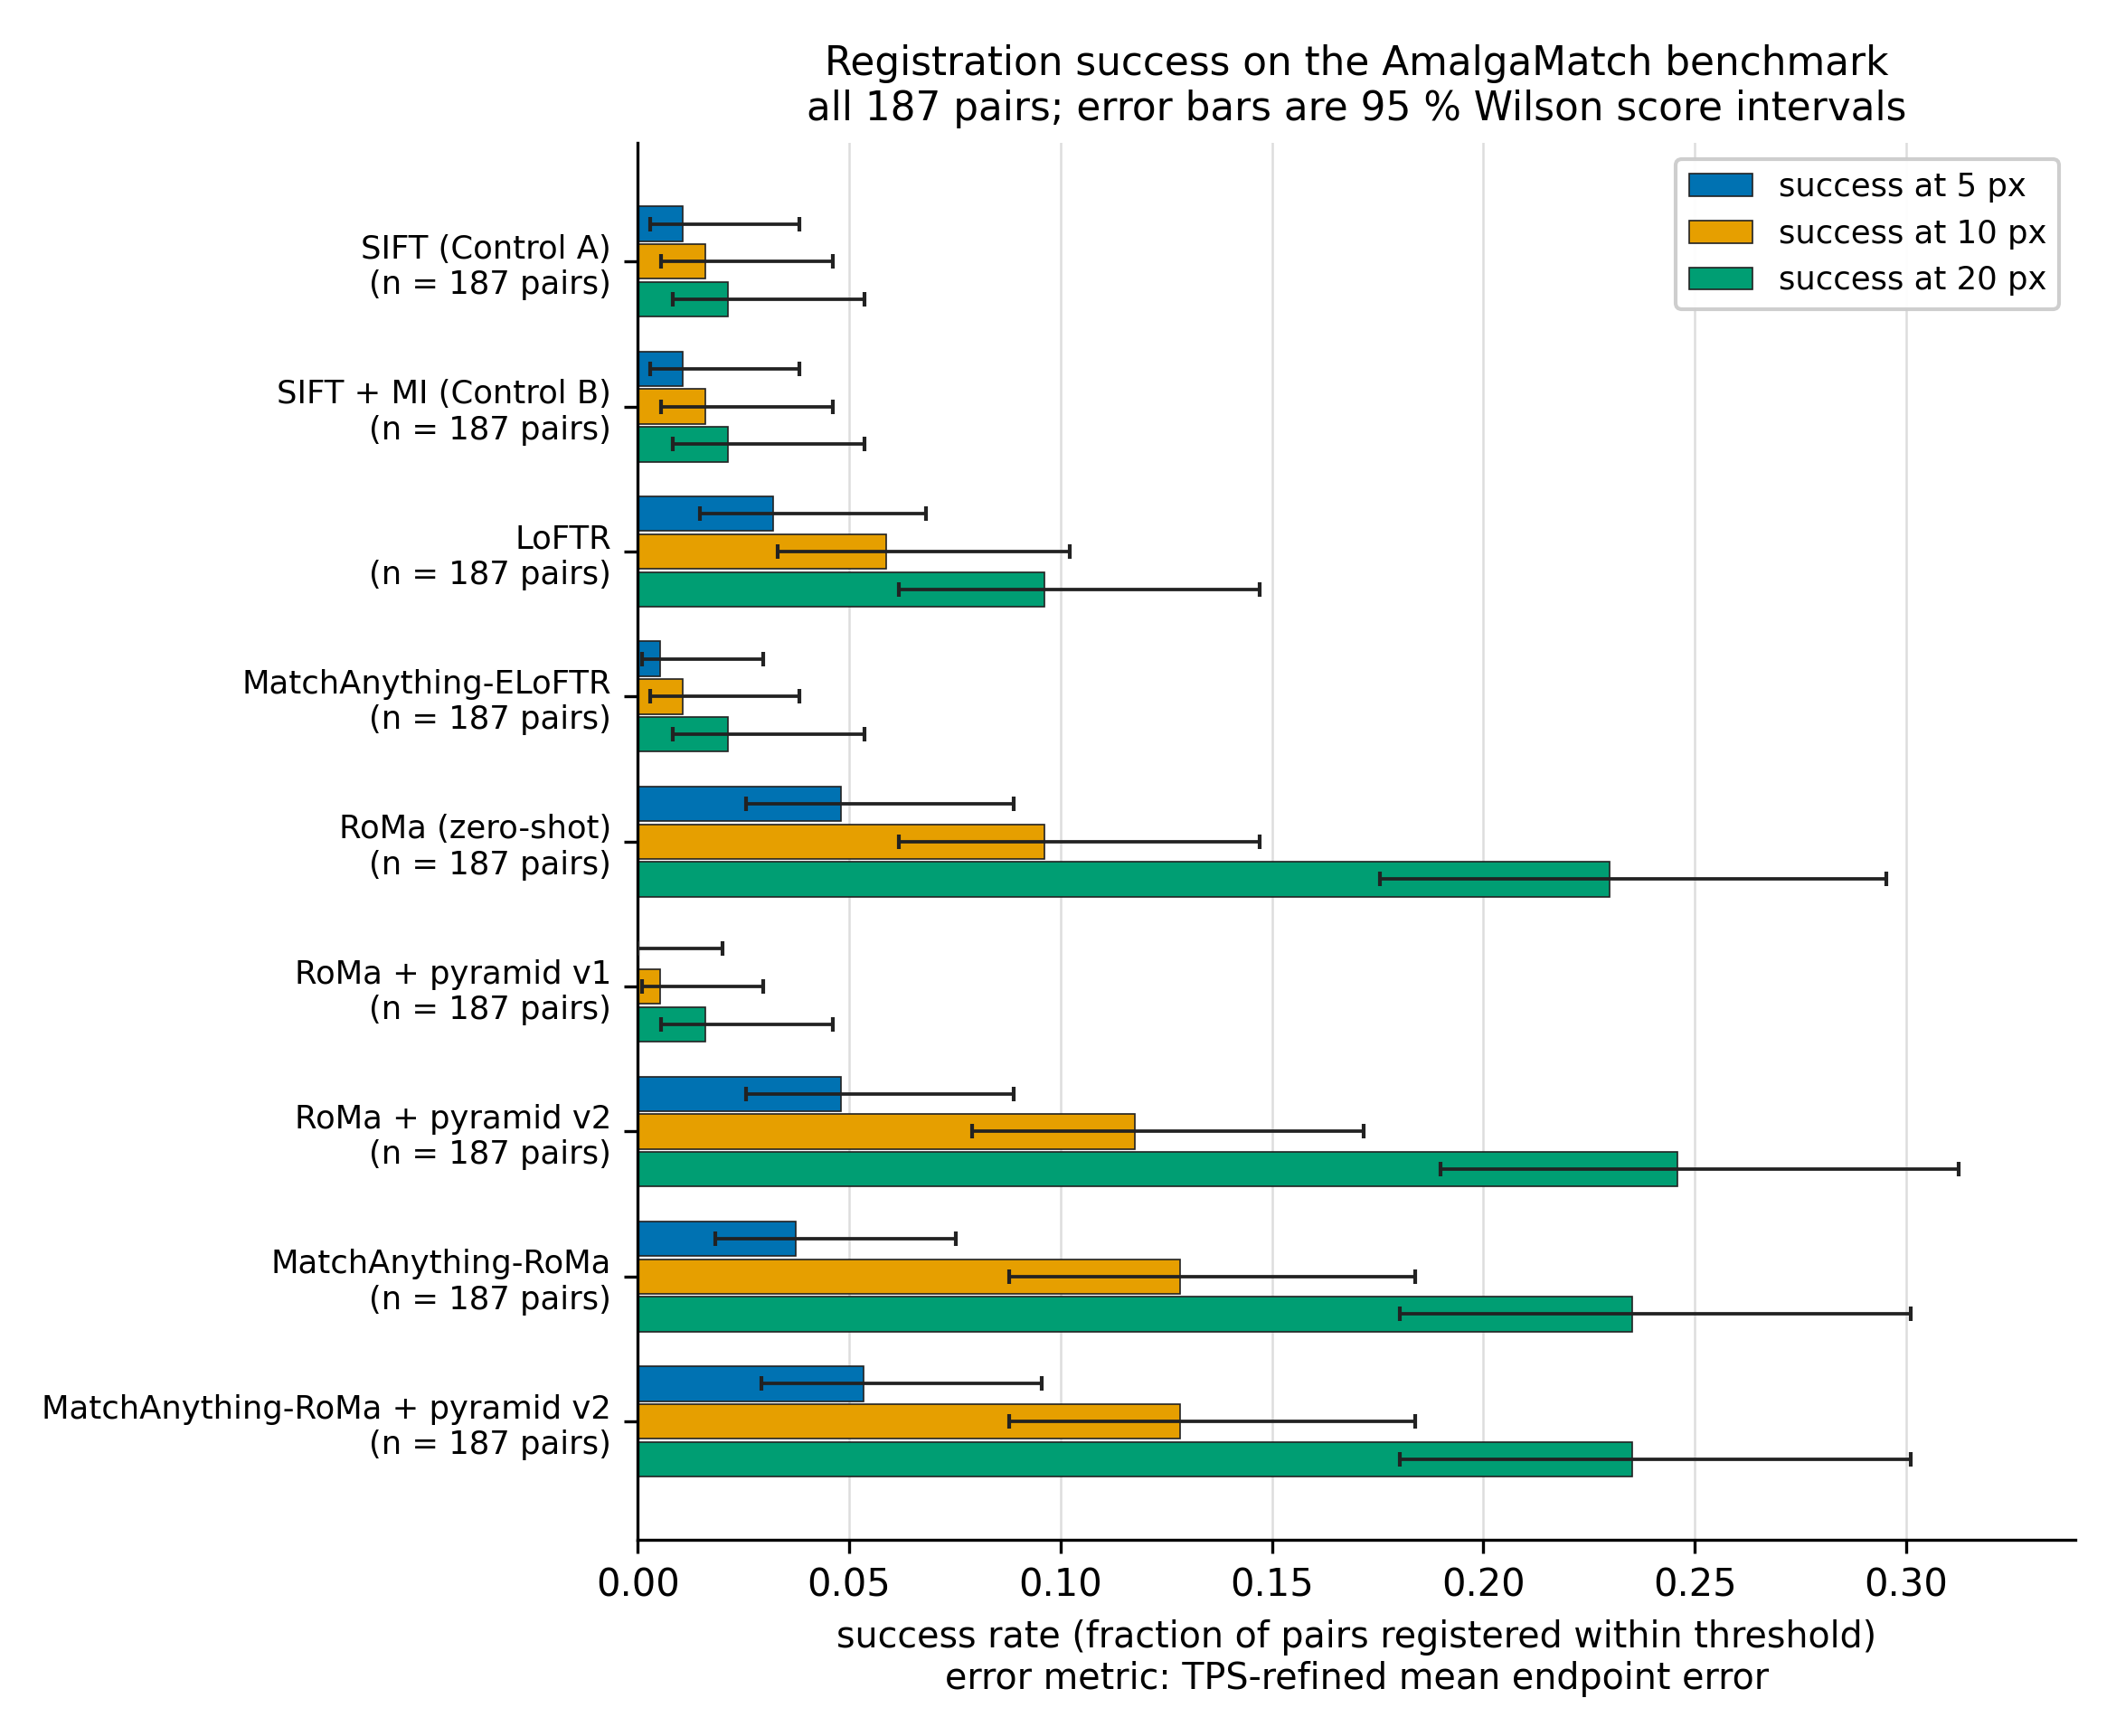
\includegraphics[width=\linewidth]{figs/sr_bars.png}
\caption{\textbf{Success rates across all configurations on AmalgaMatch.} Pyramid v1 collapses RoMa; pyramid v2 recovers a small significant gain without losing pairs; the MatchAnything-RoMa backbone provides the only significant headline gain over the zero-shot bar.}
\label{fig:srbars}
\end{figure}

\begin{figure}[ht]
\centering
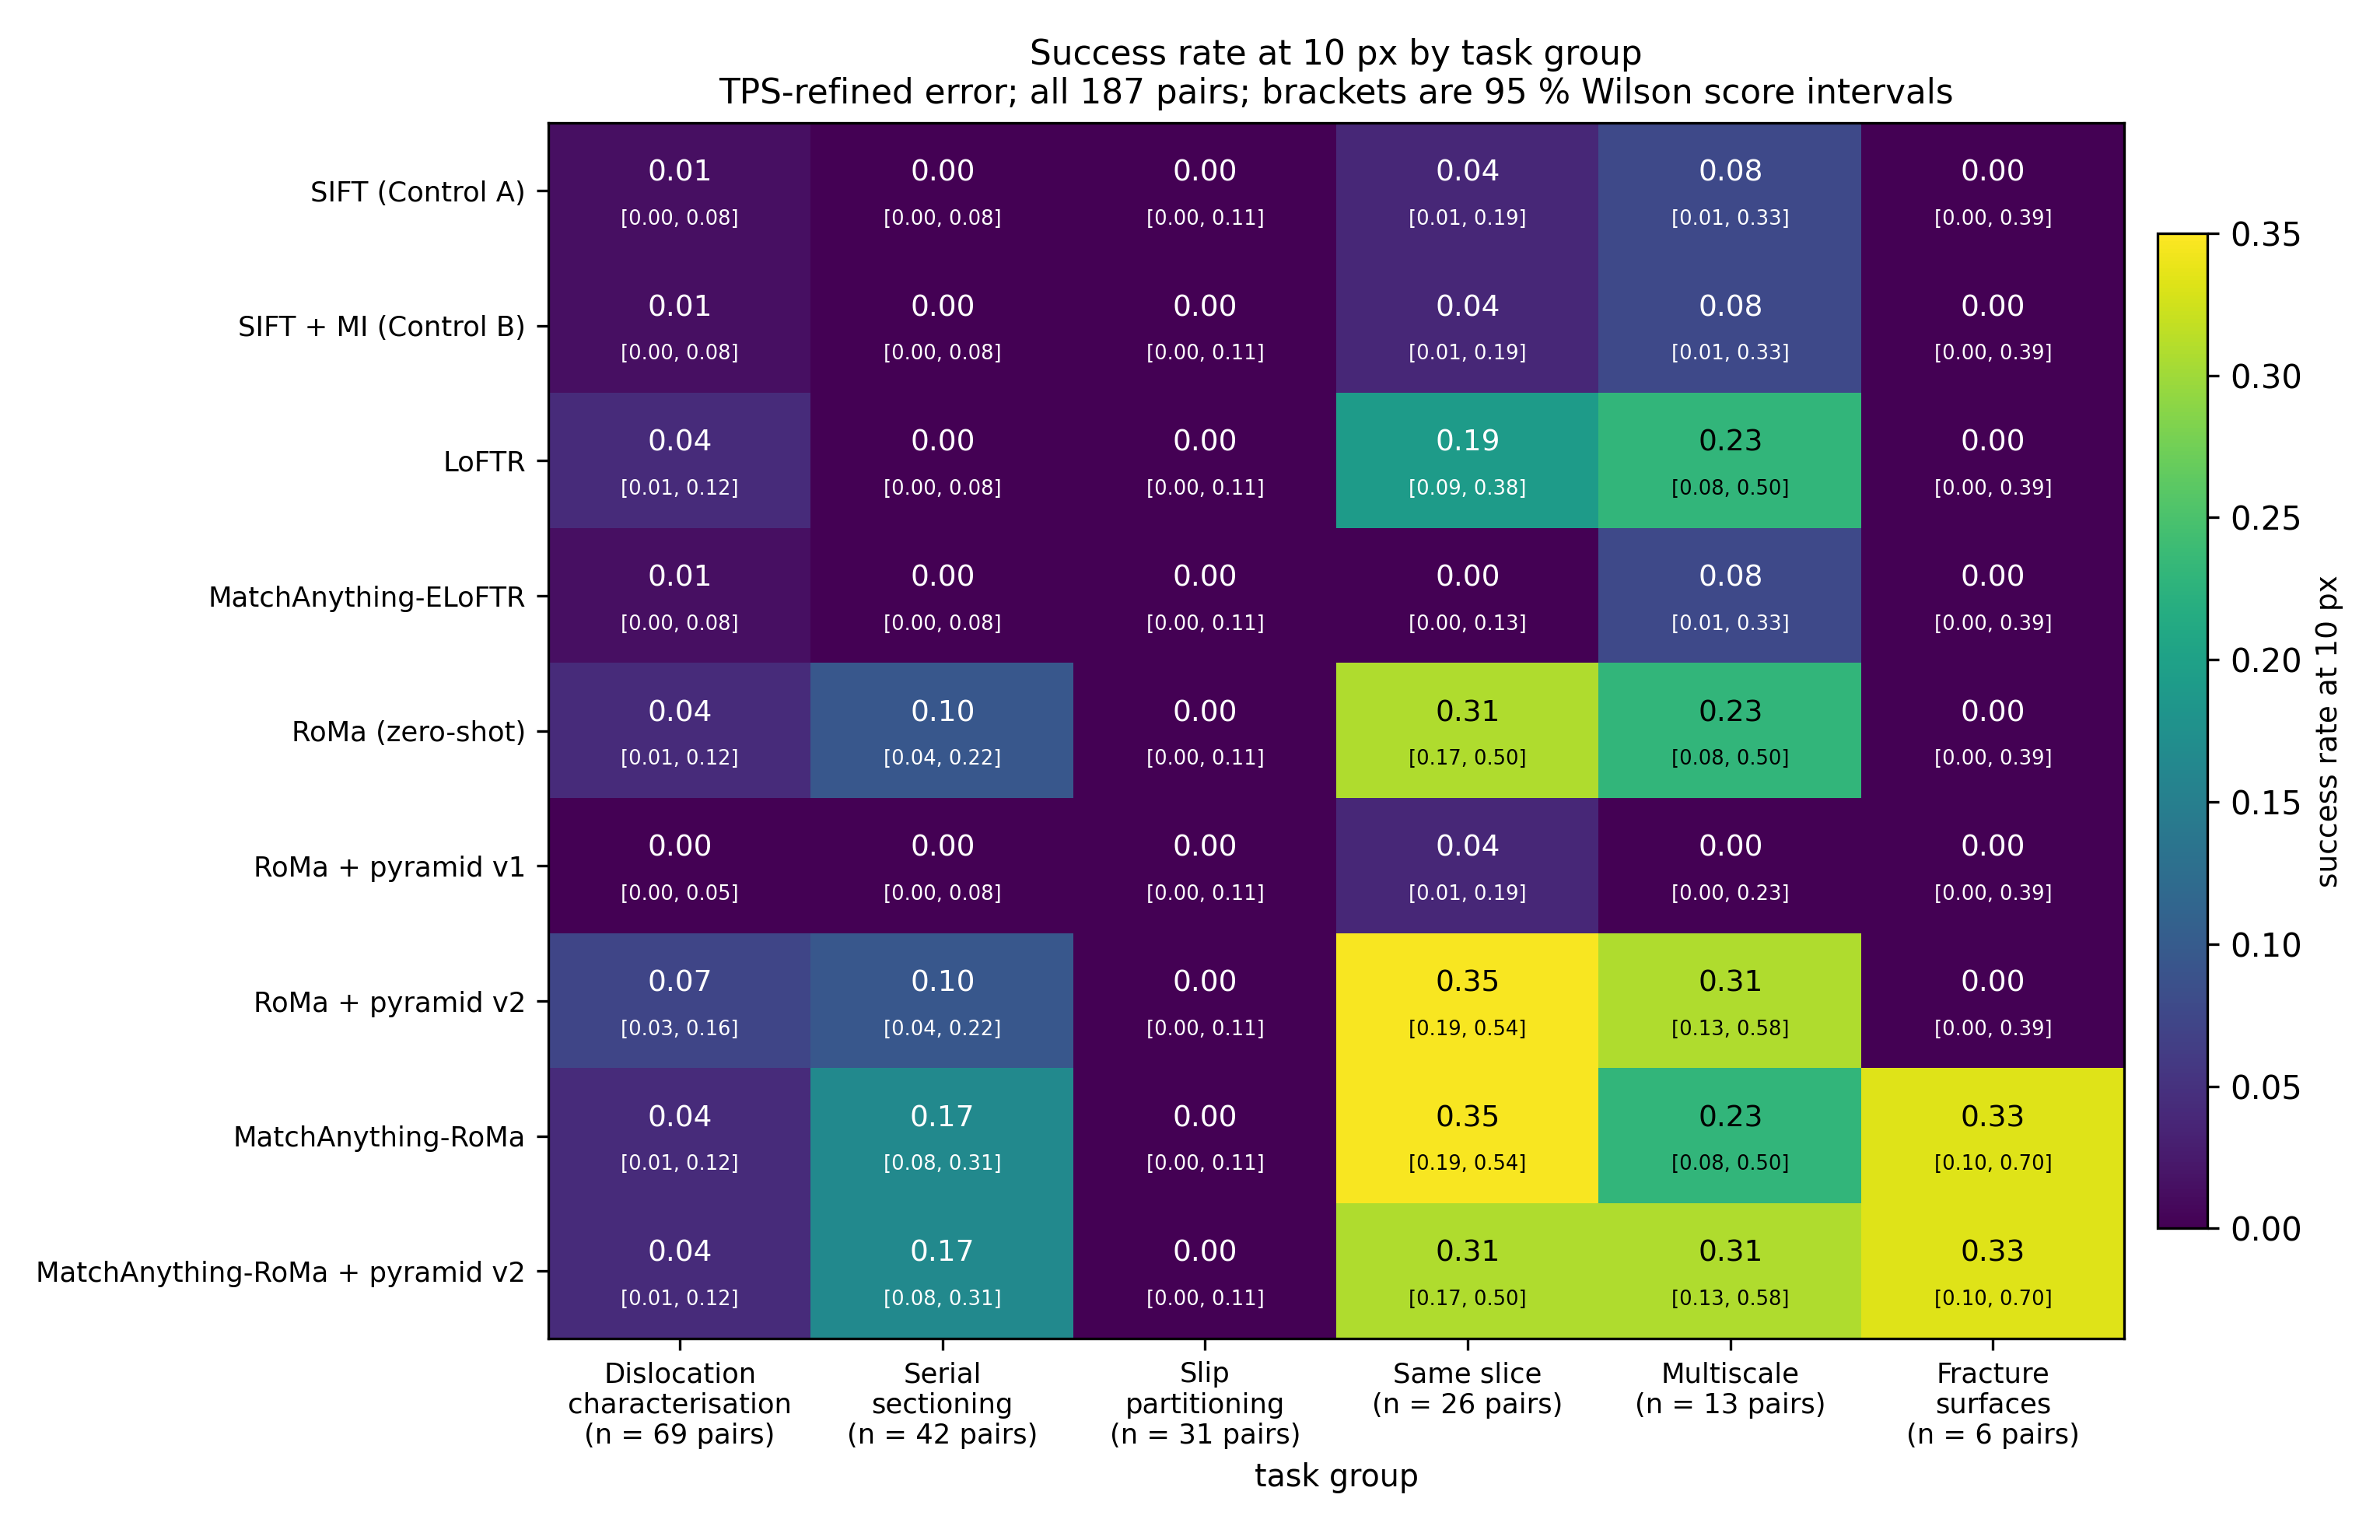
\includegraphics[width=\linewidth]{figs/group_heatmap.png}
\caption{\textbf{Per-task-group success rates.} Performance is concentrated in orientation-mapping and serial-sectioning groups; dislocation characterisation and low-mutual-information pairs remain hard for every configuration, consistent with appearance (not scale) being the dominant constraint.}
\label{fig:heatmap}
\end{figure}

\begin{figure}[ht]
\centering
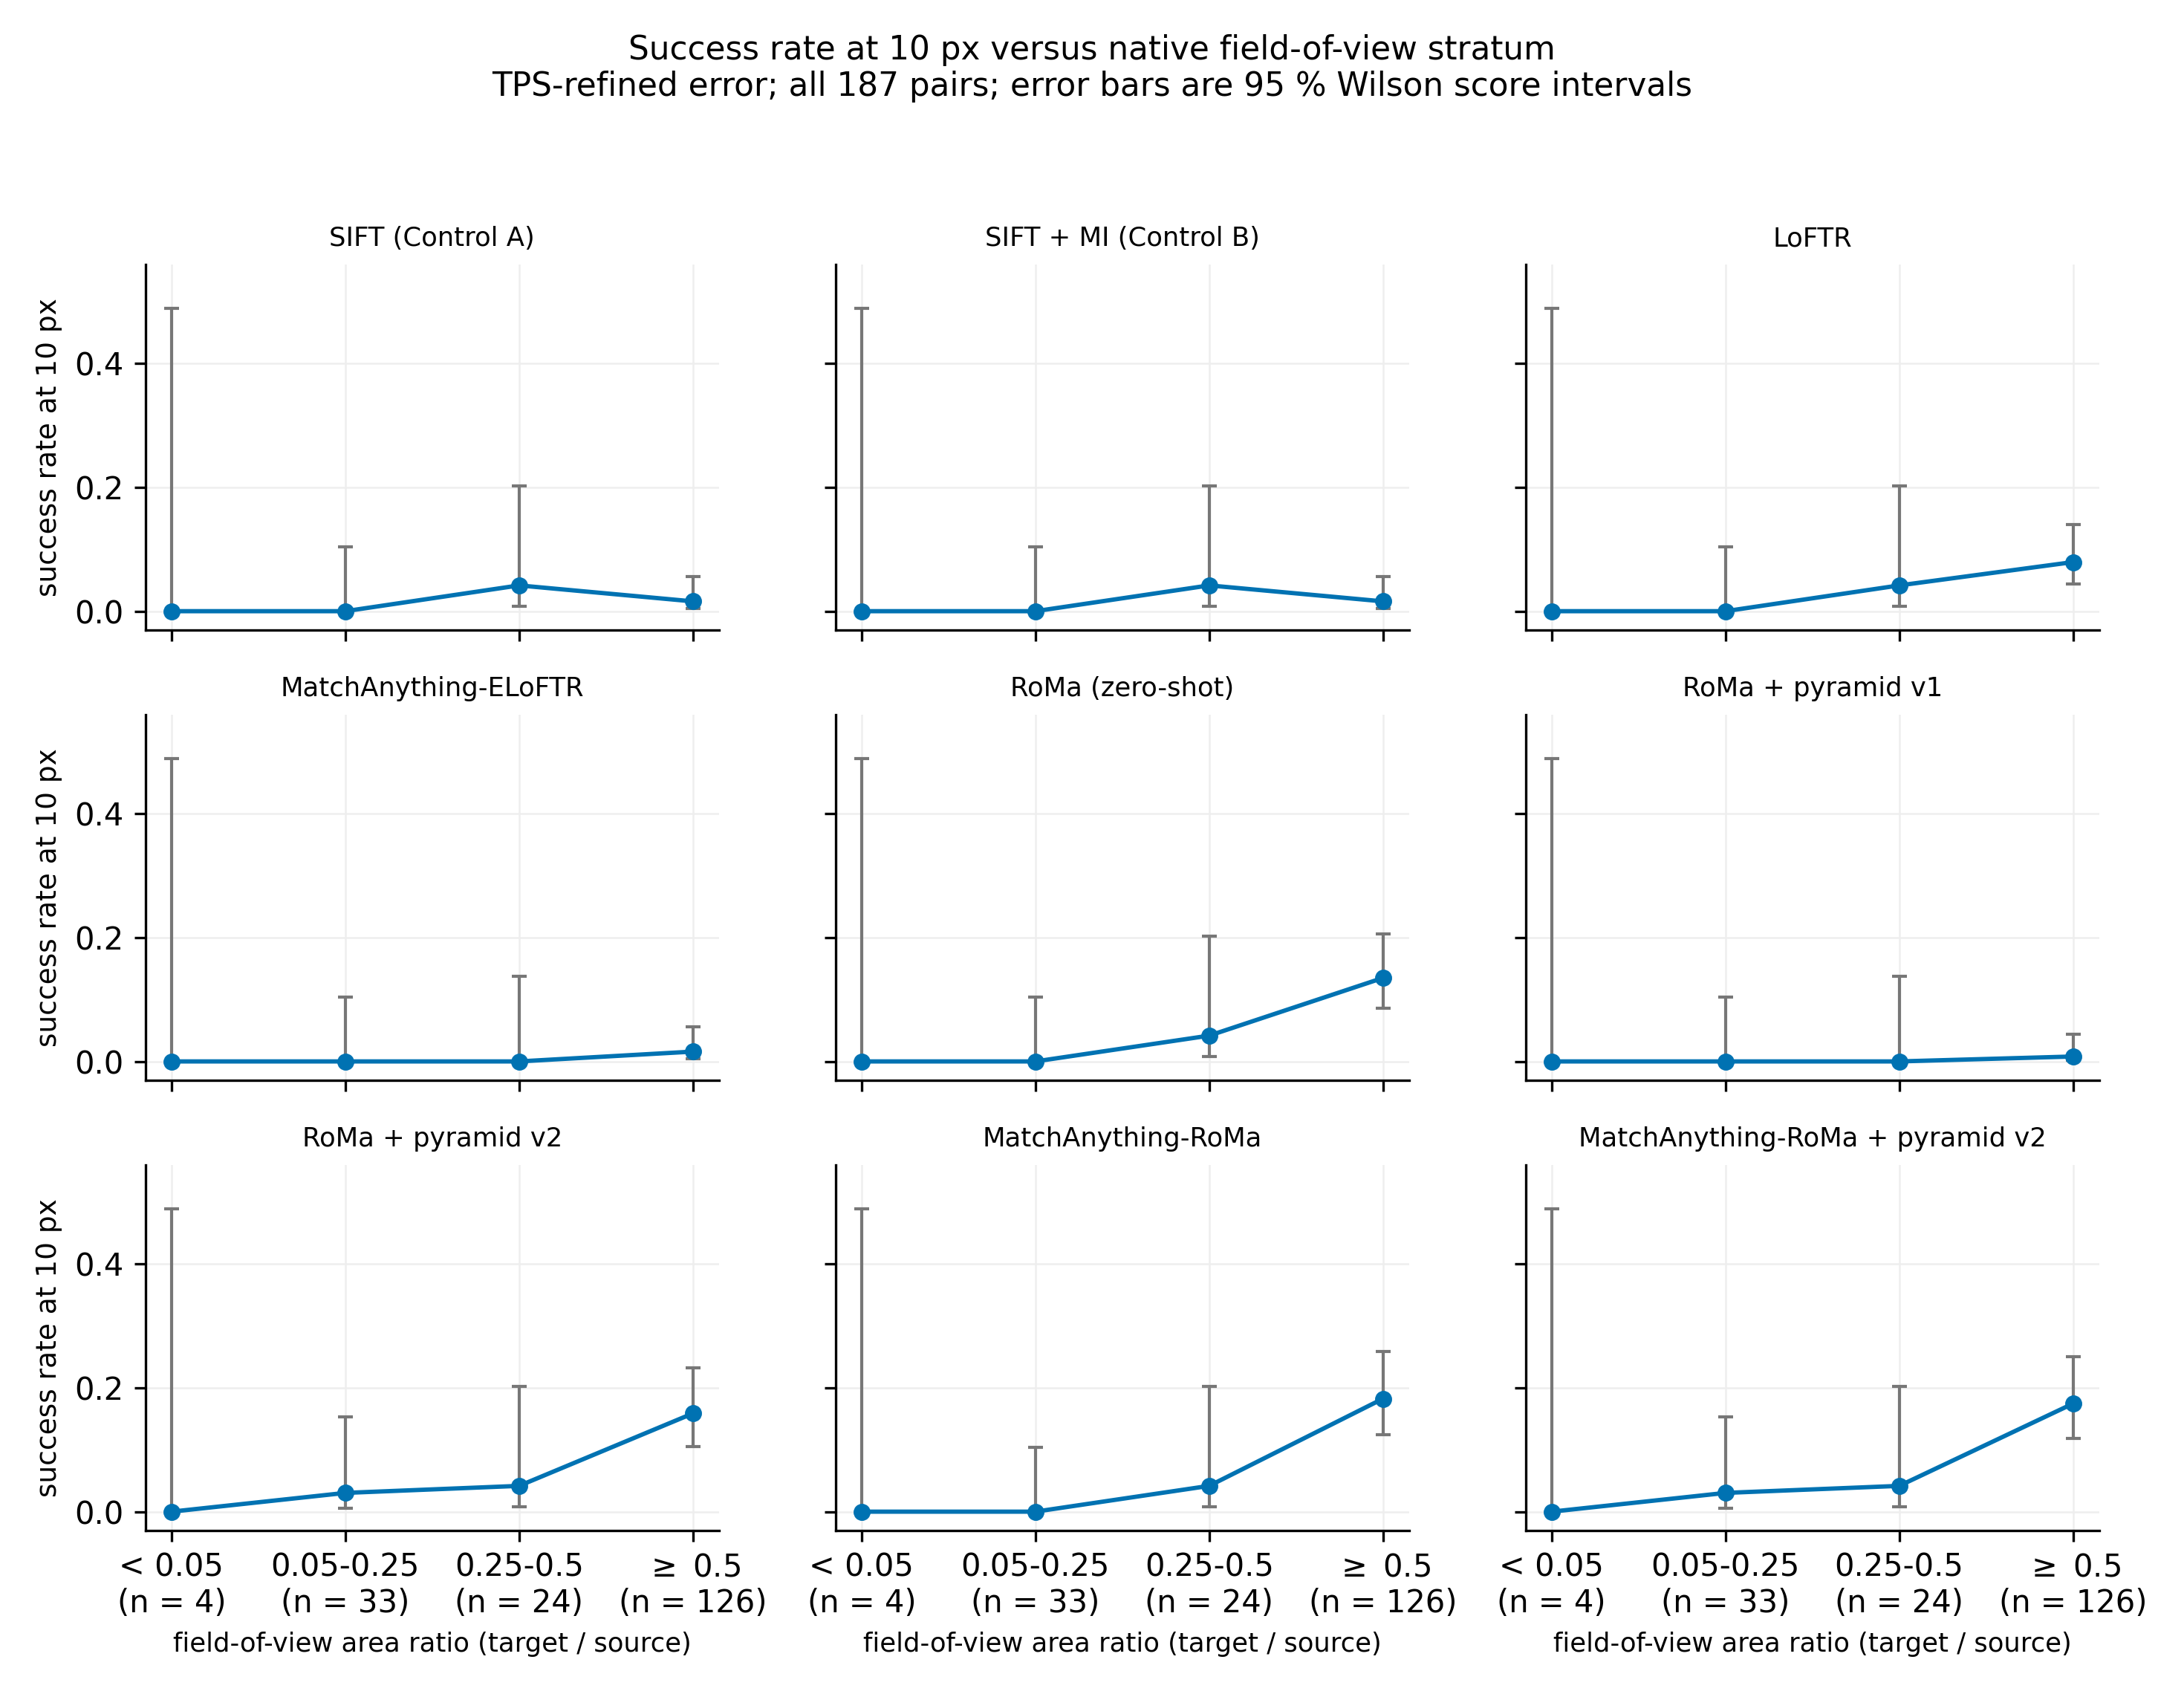
\includegraphics[width=\linewidth]{figs/fov_curves.png}
\caption{\textbf{Success rate versus field-of-view stratum on native pairs.} On the real distribution, low-FOV strata are simultaneously the most appearance-divergent, confounding scale and appearance; severe-FOV success is at the floor for every configuration.}
\label{fig:fovcurves}
\end{figure}

\begin{figure}[ht]
\centering
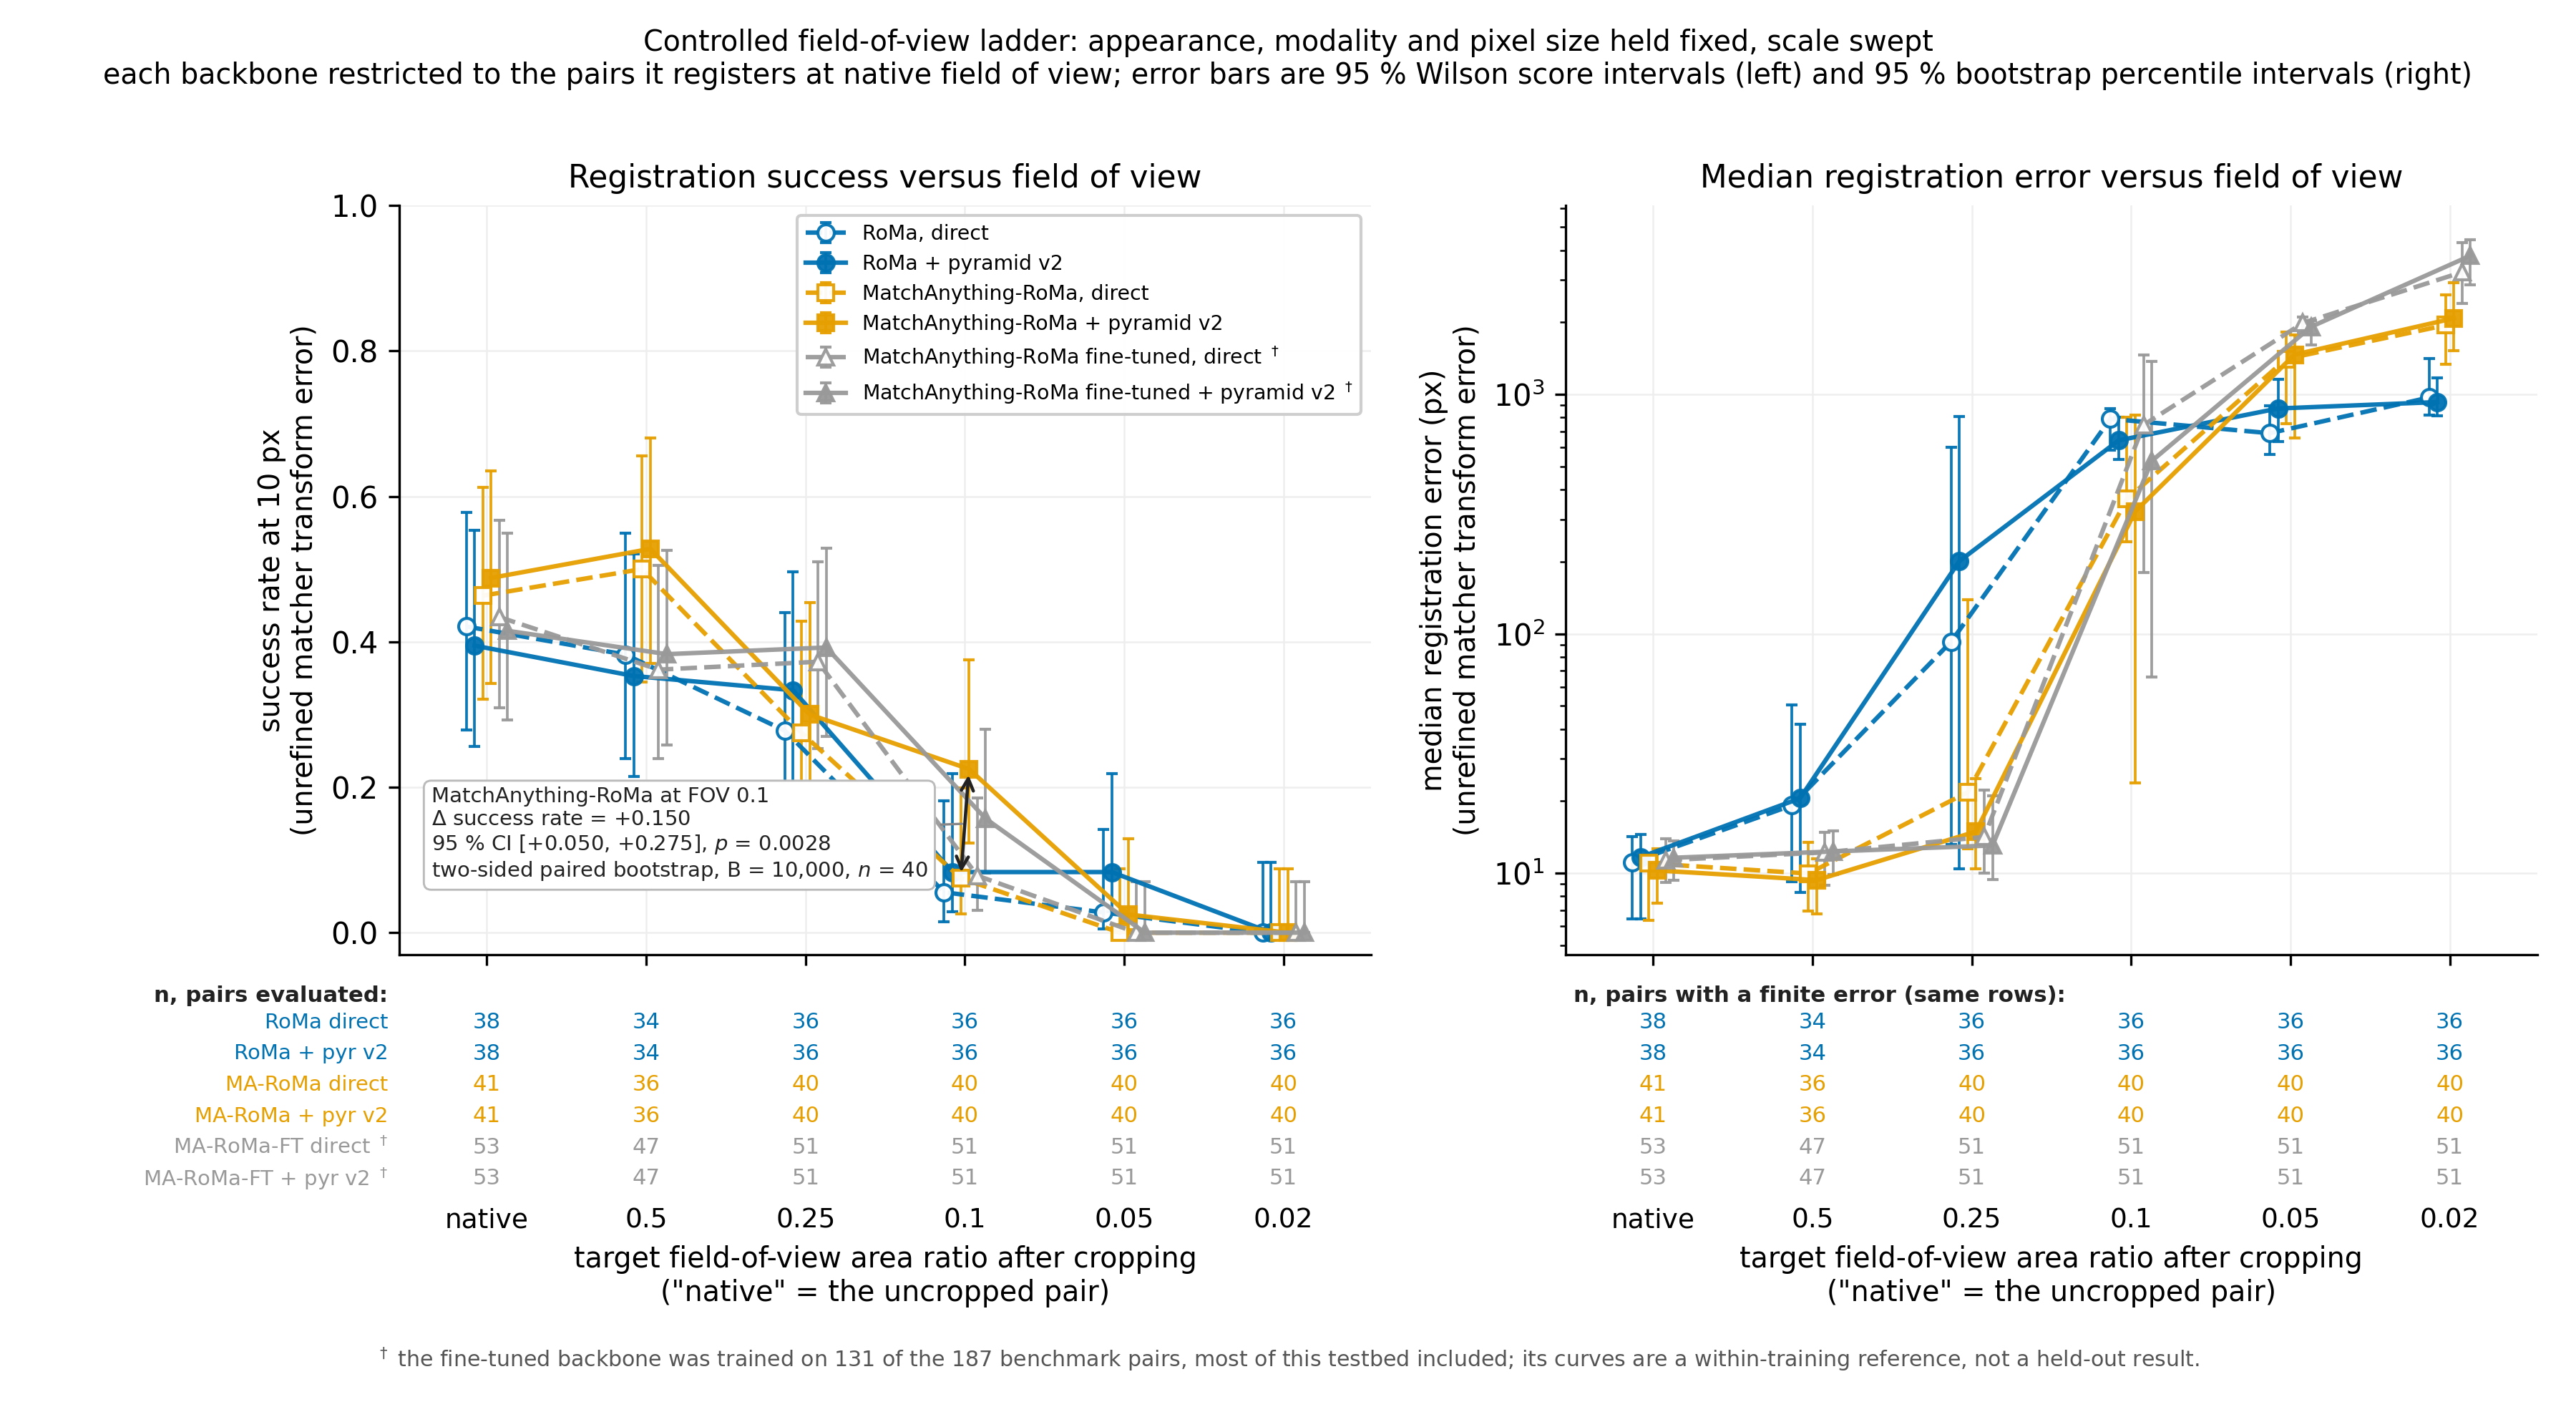
\includegraphics[width=\linewidth]{figs/fov_ladder.png}
\caption{\textbf{Controlled FOV ladder with appearance fixed.} Cropping base-matchable pairs to shrinking FOV ratios shows direct matching collapsing between 0.25 and 0.1, while the verified wrapper restores SR@10 at the 0.1 rung ($0.07\rightarrow0.23$, $p=0.0014$)---the wrapper's scale mechanism is sound once scale is isolated.}
\label{fig:fovladder}
\end{figure}

\bibliography{references}

\section*{Data availability}
The AmalgaMatch dataset is publicly available from the Fraunhofer Fordatis repository (\href{https://doi.org/10.24406/fordatis/436}{doi:10.24406/fordatis/436})\cite{durmaz2026amalgamatch}. The analysis code, evaluation harness, and result-regeneration scripts are openly available at \url{https://github.com/fronkt/correlative-microscopy-alignment}; all tables and figures regenerate from the released result files via the scripts referenced therein. Fine-tuned model checkpoints (445\,MB) are available from the author on reasonable request.

\section*{Code availability}
All code is released under the repository above. The verified coarse-to-fine wrapper, FOV-ladder construction, fine-tuning trainer, and L2-SP anchoring are provided with a single-command evaluation entry point and a synthetic-pair acceptance test.

\section*{Acknowledgements}
The author thanks the AmalgaMatch authors for releasing the dataset and the developers of RoMa, MatchAnything, Efficient LoFTR, and MAGSAC++ for releasing their code and weights.

\section*{Author contributions statement}
F.C. conceived the study, implemented the methods, conducted the experiments, analysed the results, and wrote the manuscript.

\section*{Competing interests}
The author declares no competing interests.

\section*{Funding}
This research received no specific grant from any funding agency in the public, commercial, or not-for-profit sectors.

\end{document}
